
\documentclass[twocolumn,aps,pre,floatfix,nofootinbib]{revtex4-2}

\usepackage{amsmath}

\usepackage{graphicx}

\usepackage{geometry}
\usepackage{hyperref}
\usepackage{ifthen}

% Define mapping from VAM keys to short titles
\newcommand{\VAMtitle}[1]{%
    \ifthenelse{\equal{#1}{VAM-0}}{VAM-0: \emph{From Einstein to the Vortex Fluid}}{%
    \ifthenelse{\equal{#1}{VAM-1}}{VAM-1: \emph{Time Dilation in 3D Æther}}{%
    \ifthenelse{\equal{#1}{VAM-2}}{VAM-2: \emph{Swirl Clocks \& Vorticity Gravity}}{%
    \ifthenelse{\equal{#1}{VAM-2.2}}{VAM-2}{%
    \ifthenelse{\equal{#1}{VAM-3}}{VAM-3: \emph{Benchmarking VAM vs GR}}{%
    \ifthenelse{\equal{#1}{VAM-4}}{VAM-4: \emph{Emergent GR from Swirl}}{%
    \ifthenelse{\equal{#1}{VAM-5}}{VAM-5: \emph{Lagrangian Unification of Gravity + EM}}{%
    \ifthenelse{\equal{#1}{VAM-6}}{VAM-6: \emph{Knotted Gauge Fields}}{%
    \ifthenelse{\equal{#1}{VAM-7}}{VAM-7: \emph{Quantum Constants to Galactic Swirl}}{%
    \ifthenelse{\equal{#1}{VAM-8}}{VAM-8: \emph{Topological Field Theory of Mass/Time}}{%
    \ifthenelse{\equal{#1}{VAM-9}}{VAM-9: \emph{Milky Way as Swirl-Knot Network}}{%
    \ifthenelse{\equal{#1}{VAM-10}}{VAM-10: \emph{Swirl-Induced Curvature}}{%
    \ifthenelse{\equal{#1}{VAM-11}}{VAM-11: \emph{Master Equation for Particle  Masses}}{%
    \ifthenelse{\equal{#1}{VAM-12}}{VAM-12: \emph{Fractal Swirl Extension}}{%
    \ifthenelse{\equal{#1}{VAM-13}}{VAM-13: \emph{Beyond Spacetime via Vorticity}}{%
    \ifthenelse{\equal{#1}{VAM-14}}{VAM-14: \emph{Topological Lagrangian}}{%
    \ifthenelse{\equal{#1}{VAM-15}}{VAM-15: \emph{Quantum Gravity via Superfluid Vorticity}}%
    {#1}}}}}}}}}}}}}}}}}%
}

% Make full reference a clickable link to \ref{VAM-x}
\newcommand{\VAMref}[1]{\hyperref[#1]{\textbf{\scriptsize\VAMtitle{#1}}}}

\usepackage[utf8]{inputenc}
\usepackage[T1]{fontenc}
\usepackage{amssymb}


\geometry{margin=1in}

\begin{document}


\title{Electromagnetic Swirl Coil Experiment in the Vortex Æther Model: \ Three-Phase Construction, Modeling, and Gravitational Lift Prediction}

\author{O. Iskandarani}

\date{\today}

\maketitle


\begin{abstract}

We present a theoretical experiment exploring gravitational lift from a three-phase “swirl coil” within the Vortex Æther Model (VAM). A specialized 3-phase electromagnetic coil is constructed as a 32-point polygonal winding with a chiral skip pattern (+11, –9) to induce structured vorticity in an idealized superfluid æther. We model the coil’s magnetic field via the Biot–Savart law and interpret it as a circulating aether flow (vorticity field) according to VAM’s swirl-gauge correspondence. Pulsed 3-phase excitation (both 50\% duty and an asymmetric $\sim$38.2\% duty waveform) is applied over input powers from 100W to 100kW. The resulting aetheric vorticity distribution is used to derive pressure gradients and a swirl curvature tensor $ \mathcal{R}\textit{ijk}$ in the incompressible, inviscid æther. From these, we compute the local gravity field $\vec{g}(\vec{r}) = -\nabla P/{\rho}{\text{æ}}$ and predict the net upward impulse (lift) generated by the coil’s swirl. In a VAM vacuum (superfluid æther of density\footnote{%
    In a similar way, the ætheric fluid density is taken as $\rho_\text{\ae}^{(\text{fluid})} = 7 \times 10^{-7}$ kg/m$^3$ (\VAMref{VAM-15}, Sec.~6.2), which defines the default physical density of the superfluid æther.
    This provides the scaling factor required to convert normalized gravitational field values into physical units of force or acceleration.\\%
% (Comment: Sets the unit system for converting simulated swirl-pressure gradients into real Newtonian impulse)%
}
$\rho_{\text{æ}}\approx 7\times10^{-7}$~kg/m$^3$) the simulations predict a small but finite gravity-like force opposing the local weight. For comparison, an air-medium simulation is included to distinguish true ætheric lift from mere aerodynamic or electromagnetic forces. The paper is organized into Introduction, Methods, Coil Design, Simulation Results, Swirl Gravity Derivation, Discussion, and Conclusion. We aim to establish a lab-testable prediction: a properly driven three-phase coil can produce a discernible gravitational lift via structured aether vorticity, thus providing experimental validation for electroswirl propulsion under VAM principles.

\end{abstract}


\section{Introduction}

General relativity attributes gravity to spacetime curvature produced by mass-energy, whereas the Vortex Æther Model reinterprets gravitation as an emergent effect of structured fluid rotation (vorticity) in a physical æther medium. In VAM, matter is modeled as stable vortex knots in an incompressible superfluid æther, and gravity arises from the pressure gradients induced by these vortex flows (a fluid-dynamic analogue of curvature) rather than by geometric warping of spacetime\footnote{%
    As introduced in \VAMref{VAM-10}, gravity in the Vortex Æther Model is not a geometric effect of curved spacetime, but a dynamical consequence of structured swirl in a superfluid æther.
    The local curvature of trajectories arises from sustained vorticity patterns that generate pressure deficits, mimicking the gravitational attraction observed in General Relativity.
    Matter, in this view, corresponds to topologically stable vortex knots, and inertial motion results from the conservation of circulation within the surrounding æther.\\%
% (Comment: Captures the core ontological reinterpretation of gravity via æther swirl, not geometric curvature)%
}. In essence, “why do things fall?” is answered in VAM by the inward push of circulating æther flow (swirl-induced pressure deficits) that curves trajectories inward. Prior VAM studies have shown that the gravitational potential $\Phi_v$ obeys a Poisson-like equation\footnote{%
    In VAM, “why do things fall?” is answered by the inward push of circulating æther flow—swirl-induced pressure deficits—that curves trajectories inward.
    Prior studies (\VAMref{VAM-2}, Sec.~3.2) showed that the gravitational potential $\Phi_v$ obeys a Poisson-like equation:
    \[
        \nabla^2 \Phi_v(\mathbf{r}) = -\rho_{\text{æ}}|\boldsymbol{\omega}(\mathbf{r})|^2,
    \]
    where $\boldsymbol{\omega} = \nabla \times \mathbf{v}$ is the vorticity of the æther flow and plays the role of mass density in generating gravity.\\%
% (Comment: Links vorticity magnitude to source term in gravitational potential equation)%
} \[\nabla^2 \Phi_v(\mathbf{r}) = -,\rho_{\text{æ}}|\boldsymbol{\omega}(\mathbf{r})|^2\], where $\boldsymbol{\omega}=\nabla\times \mathbf{v}$ is the vorticity of the æther flow and plays the role of mass density in generating gravity. A rapidly rotating vortex thus creates a low-pressure region which acts as a gravitational potential well, drawing objects inward (or, equivalently, “downward”) toward the vortex core. This fluid-based mechanism reproduces Newtonian gravity and frame-dragging in the appropriate limits, while also providing novel insights into gravitational time dilation and other phenomena as consequences of swirl dynamics\footnote{%
    This follows the time dilation formalism derived in \VAMref{VAM-2.2}, Sec. 2.2,
    where swirl clocks are shown to dilate local time proportionally to the
    squared vorticity magnitude: $d\tau = dt \sqrt{1 - |\vec{\omega}|^2 / c^2}$.\\%
% (Comment: This footnote links vorticity to proper time, used to justify gravity via Bernoulli pressure)%
}.


The idea of generating artificial gravity or weight reduction via rotation has a long history. Notably, Podkletnov & Nieminen (1992) reported anomalous weight losses (on the order of $0.3\%$–$2\%$) above a rapidly spinning superconducting disc in a magnetic field \cite{Podkletnov1992}. Although controversial, such results hint that electromagnetic rotation might influence gravity under special conditions. Conventional physics has struggled to explain these claims, since a rotating magnetic field or superconducting lattice should produce negligible gravitational effects in general relativity (the energy densities are far too small). However, within VAM, a possible explanation emerges: the superconductor and magnetic field setup could have induced a persistent aether vortex (a quantized swirl) with a corresponding pressure deficit above the disc, leading to a slight reduction in weight. This motivates exploring electromagnetic systems that deliberately generate structured vorticity in the æther. If VAM is correct, even a purely electromagnetic apparatus (with no massive moving parts) could produce a gravity-like force by creating a dynamic pattern of aether swirl.


In this paper, we propose a three-phase “swirl coil” experiment as a practical test of VAM’s predictions. The concept is to use a specially wound coil driven by phased AC currents to produce a rotating magnetic field in free space. According to VAM’s electromagnetism–swirl duality, a magnetic field corresponds to circulation of the æther\footnote{%
    As outlined in \VAMref{VAM-14}, Sec.~2.2, magnetic fields are reinterpreted as manifestations of circulating flow within the æther — specifically, as topologically constrained vorticity tubes in a superfluid medium.
    This reformulation replaces the field-line abstraction with physical swirl structures governed by fluid momentum conservation.
    In this duality, the vector potential $\vec{A}$ becomes a proxy for swirl velocity, and $\vec{B} = \nabla \times \vec{A}$ reflects the local ætheric vorticity.
    Therefore, driving an AC coil to create a rotating $\vec{B}$-field corresponds directly to injecting angular momentum into the æther, forming a sustained vortex structure.\\%
% (Comment: Establishes the EM-to-vorticity mapping used to justify the swirl coil as a physical vortex injector in VAM)%
}, so a rotating magnetic field should induce a rotating aether flow (i.e. a vortex). By arranging the coil geometry and drive signals to concentrate this swirl, we aim to generate a vertical pressure gradient in the æther analogous to a vortex column, which would manifest as an upward “lift” force on nearby masses or on the coil itself. The resulting effect can be viewed as an electrodynamic version of a tornado: just as a tornado’s swirling air can lift objects via low pressure at its core, a swirling æther flow might produce a gentle anti-gravity effect.


The following sections detail the coil design, the modeling methods used to compute the magnetic (swirl) field and resulting gravitational field, and the outcomes of simulations across a range of input powers and duty cycles. We then discuss experimental considerations for detecting the predicted lift, and how a successful demonstration would provide evidence for the VAM framework. This work bridges the gap between theoretical vortex gravity and laboratory engineering, offering a concrete test of the VAM idea that gravity can be generated (and potentially controlled) via electromagnetic means — a concept we term \textit{electroswirl propulsion}.


\section{Methods}

Our approach combines electromagnetic field simulation with fluid dynamic analogues as prescribed by VAM. First, we compute the magnetic field of the three-phase coil using the Biot–Savart law and superposition of time-phase currents. The coil’s current distribution is broken into a set of filamentary segments, and the magnetic flux density $\mathbf{B}(\mathbf{r})$ is obtained by integrating \[\mathrm{d}\mathbf{B} = \frac{\mu_0 I}{4\pi}\frac{d\mathbf{l}\times \hat{\mathbf{r}}}{r^2}\] over all segments for a given instantaneous current $I$ in each phase. We perform this calculation for each phase excitation state in the 3-phase cycle, effectively mapping out the rotating magnetic field pattern produced by the coil. The simulation is run for two duty cycle regimes of the pulse-width modulated (PWM) drive: a symmetric 50\% duty (square-wave excitation) and an asymmetric $\approx 38.2\%$ duty chosen for its relation to the golden ratio (discussed below). The input power is varied from 0.1kW up to 100kW, and at each power level the current amplitude is adjusted according to the coil’s impedance to maintain the specified power (accounting for resistive heating losses in the wire).


Second, we translate the magnetic field results into an ætheric vorticity field. In VAM’s formulation of electromagnetism, the magnetic field $\mathbf{B}$ is identified with the curl of an aether velocity field (i.e. vorticity)~\cite{Barcelo2011}. We thus treat the magnetic flux distribution $\mathbf{B}(\mathbf{r},t)$ obtained from Biot–Savart as proportional to the aether’s vorticity $\boldsymbol{\omega}(\mathbf{r},t) = \nabla \times \mathbf{v}\textit{\text{æ}}$. In physical terms, the coil’s oscillating currents induce a swirling motion in the invisible æther medium: wherever $\mathbf{B}$ loops or curls, the aether is circulating. The proportionality constant between $\mathbf{B}$ and $\boldsymbol{\omega}$ can be considered an experimental coupling factor (in a simple analogy, one might imagine $\mathbf{v}_{\text{æ}}$ having units of velocity such that $\rho_{\text{æ}}\mathbf{v}_{\text{æ}}$ corresponds to a momentum density analogous to the magnetic field energy density). For the purpose of this theoretical study, we focus on the shape and relative strength of the induced swirl, rather than its absolute scale, noting that higher coil currents (and/or using high-permeability cores) would amplify the magnitude of $\boldsymbol{\omega}$. Each phase in the coil contributes a vector vorticity field, and the 120$^\circ$ phase-shifted AC drives ensure that the total $\boldsymbol{\omega}(\mathbf{r},t)$ rotates in space as a function of time, maintaining a approximately constant-magnitude swirling pattern that simply changes orientation (a “rotating vortex”). We capture this behavior by sampling the vorticity field at discrete time steps corresponding to the PWM cycle states (+–0, –0+, 0+– described below) and by analytically confirming that the time-average vorticity is nonzero and chiral (i.e. it consistently circulates in one direction).


Third, given the aetheric vorticity $\boldsymbol{\omega}(\mathbf{r})$, we derive the resultant pressure field using a Bernoulli-like relation appropriate for steady rotational flows. For an incompressible, inviscid fluid, the steady-state Euler equation gives $\nabla P = -\rho_{\text{æ}},(\mathbf{v}\cdot\nabla)\mathbf{v}$; in a purely swirling flow, this leads to lower pressure in regions of higher vorticity (in order to centripetally confine the swirl). We integrate these relations or, equivalently, apply Bernoulli’s theorem (which in the presence of rotational flow yields $P+\frac{1}{2}\rho_{\text{æ}}v^2=\text{const}$ along streamlines). Thus, wherever the coil induces a high rotational speed $v_{\text{æ}}$, we expect a pressure deficit $P$ relative to the far-field ambient. The pressure $P(\mathbf{r})$ is computed by assuming a reference pressure $P_0$ at the outer boundary of our simulation domain (far from the coil, where flow is negligible), and subtracting the dynamic pressure $\frac{1}{2}\rho_{\text{æ}} v_{\text{æ}}^2(\mathbf{r})$ for each point. This yields a 3D pressure map $P(x,y,z)$ in the region around the coil. We perform this calculation for the coil oriented in the horizontal ($xy$) plane with its axis vertical ($z$). The pressure solution reveals a characteristic low-pressure column along the axis of rotation (above the coil center) due to the induced swirl, analogous to the “eye” of a vortex.


Fourth, we calculate the local gravitational acceleration field\footnote{%
    The gravitational acceleration $\vec{g} = -\vec{\nabla} P / \rho_\text{\ae}$ is derived in
    \VAMref{VAM-10}, Sec. 4.1, where the æther pressure gradient arises from rotational swirl energy.%
% (Comment: This footnote justifies using pressure gradients from vorticity as gravitational acceleration)%
} as \[\vec{g}(\vec{r}) = -\nabla P(\vec{r})/\rho_{\text{æ}}\]. This formula stems directly from the Euler equation in a static vortex: a pressure gradient is the source of acceleration (force per unit mass) on a test particle. In VAM, $\vec{g}$ is interpreted as the emergent gravitational field. We anticipate that $\vec{g}$ will point inward toward regions of lower pressure. In the context of our coil, that means $\vec{g}$ has an upward vertical component above the coil (since pressure is lowest along the axis just above the coil) and perhaps a slight inward horizontal component toward the symmetry axis. We compute $\vec{g}$ by taking finite differences of the $P$ field. Furthermore, to quantify the total lift force, we integrate the pressure over a horizontal plane above the coil (or equivalently integrate $\rho_{\text{æ}}\vec{g}$ over the volume to get momentum flux). In practice, an easier estimate of net lift $F_{\text{lift}}$ is obtained by integrating the vertical pressure force on the coil or on an imaginary “lid” over the coil: \[F_{\text{lift}} \approx \iint (P_{\text{below}} - P_{\text{above}}),dA\], where $P_{\text{below}}$ is ambient (no swirl under the coil) and $P_{\text{above}}$ is reduced by swirl. Since $P_{\text{above}} < P_{\text{below}}$, this pressure difference times area yields an upward force. We perform this integration across the area roughly corresponding to the coil’s footprint (assuming the swirl primarily affects a column above the coil of radius similar to the coil radius).


Fifth and finally, we consider two medium cases: (a) the ideal VAM vacuum, where $\rho_{\text{æ}}\approx7\times10^{-7}$~kg/m$^3$ and the fluid is nonmaterial (no air drag or heating), and (b) a control case with the coil operating in normal air (with $\rho_{\text{air}}\approx1.2$kg/m$^3$ and standard viscosity). The air case is included to generate a secondary plot of pressures and flow, illustrating that any measured lift in an actual experiment must be distinguished from trivial aerodynamic effects. In the air simulation, the same coil currents will produce a rotating magnetic field but also induce some air motion (via coupling to ionized particles or thermal convection due to coil heating). However, without actual spinning blades, any airflow is minimal; thus a significant lift in vacuum that cannot be explained in the air case would strengthen the interpretation of an ætheric effect. In both cases, we normalize the output lift force against the input electrical power to obtain a “lift efficiency” (Newtons of lift per watt). We also account for coil impedance and losses: at high power, the coil may heat significantly and its resistance can increase, reducing current for a given drive voltage. Our modeling includes a simple $R + j\omega L$ impedance calculation to adjust current amplitude with frequency and to estimate the fraction of input power actually going into electromagnetic field (vs Joule heating). For consistency, all simulations are run at a nominal frequency of 50Hz (mains frequency), though frequency can be varied; the rotation of the magnetic field (and thus the swirl) is locked to the drive frequency.


Throughout these steps, computational tools were used to solve field distributions. Custom Python code was written to evaluate the Biot–Savart integrals and to perform finite-difference operations on a spatial grid for $\nabla P$. Convergence was checked by refining the spatial grid until changes in peak $\vec{g}$ were below 1\%. No gravity-like effect was inserted manually; the emergence of $\vec{g}\neq 0$ is purely a result of the coil’s creation of a structured $\boldsymbol{\omega}$ field in the VAM framework.


\section{Coil Design}

The coil is designed specifically to maximize a net chiral aether swirl while minimizing symmetry that could cancel out pressure gradients. We choose a base geometry of a 32-corner polygon (an approximation of a circle) as the winding path for the coil. The wire is routed such that it connects every 32nd corner in a repeating skip pattern of “forward 11, back 9.” In practice, this means if we number the corner points $0,1,2,\dots,31$ around the loop, the wire goes from point $i$ to point $i+11$ (mod 32) for one segment, then from that point to $i+11-9 = i+2$ (mod 32) for the next segment, then again forward by 11, and so on. This +11/–9 sequence creates a starpolygon-like winding that wraps around the circle multiple times before closing, ensuring the coil’s current crosses the interior in a highly twisted manner. The resulting winding has a pronounced chirality: it is not simply a circular loop, but a helical swirl that repeatedly advances around the coil while also doubling back. The forward vs backward skip count (11 vs 9) are chosen to be asymmetric (producing a net +2 advance per two segments) so that the pattern covers the entire 32-point loop in one continuous wire without mirror symmetry. In essence, the coil is a single-loop Möbius-like winding that densely fills a donut-shaped surface with current in a way that all current flow has a consistent rotational sense (either clockwise or counter-clockwise when viewed from above). This geometry was arrived at to concentrate magnetic flux (and thus aether swirl) near the center. By comparison, a simple circular loop or even a dense solenoid winding might produce strong fields but much of the vorticity would be axisymmetric and could cancel out net forces. The introduced asymmetry enforces a one-directional bias in the field structure.


To further concentrate the swirl, multiple layers of this 32-point winding can be stacked\footnote{%
    The layered coil geometry and z-axis swirl amplification follow \VAMref{VAM-12}, Sec. 2.5,
    where fractal phase-stacked vortices produce enhanced swirl curvature in confined regions.%
% (Comment: This footnote supports the coil design strategy: stacking → increased curvature → stronger lift)%
}
vertically (along the coil’s $z$ axis). We envision three layers tightly sandwiched (such that the vertical spacing between layers is much smaller than the coil radius). Each layer carries one phase of the 3-phase current. For example, PhaseA could occupy the bottom layer, PhaseB the middle, Phase~C the top. All layers use the same +11/–9 path, aligning corner points above each other. By energizing the phases in sequence, the combined effect is a swirling magnetic field that extends upward from the coil. The vertical stacking is critical: it forces the magnetic (and aetheric) field lines from each layer to interact and “twist” the aether in a concentrated column. Essentially, we are creating a short, thick vortex coil as opposed to a tall solenoid—the goal is a tight toroidal field structure whose center has intense curl.


The three-phase excitation is implemented using a $120^\circ$ stepped driving sequence, denoted as $(+;\,-;\,0)$, $(-;\,0;\,+)$, and $(0;\,+;\,-)$. Here, “\(+\)” indicates that the respective phase's current is at positive peak (flowing in the defined forward winding direction), “\(-\)” indicates negative peak (reverse flow), and “0” indicates that the phase is at zero crossing or inactive. This discrete 3-step sequence approximates the continuous sinusoidal progression of a standard three-phase AC drive and repeats cyclically as a rotating excitation pattern.

\begin{table}[h]
    \centering
    \begin{tabular}{c|c c c}
        \toprule
        \textbf{Step} & \textbf{Coil A} & \textbf{Coil B} & \textbf{Coil C} \\
        \midrule
        1 & \(+\) & \(-\) & \(0\) \\
        2 & \(-\) & \(0\) & \(+\) \\
        3 & \(0\) & \(+\) & \(-\) \\
        \bottomrule
    \end{tabular}
    \caption{Three-step phase excitation sequence for the swirl coil. Each row shows the drive polarity applied to the three coils (A, B, C) during one step of the cycle. The pattern rotates cyclically to induce a unidirectional vortex in the æther.}
    \label{tab:3-phase-steps}
\end{table}

At each step in the cycle, a pair of coils carry equal and opposite current (\(\pm I\)) while the third is idle. For example, during step 1, Coil A carries \(+I\), Coil B carries \(-I\), and Coil C is off. This rotates to step 2, where Coil A has \(-I\), Coil C has \(+I\), and Coil B is zero, and so on. The resulting $(+\!-\!0 \rightarrow -\!0\!+ \rightarrow 0\!+\!-\rightarrow \cdots)$ sequence drives a chiral rotating magnetic field, acting as a pulsed vortex injector into the surrounding æther medium.
 This stepping drive is akin to the commutation sequence of a brushless DC motor, but here we emphasize the generation of a smooth rotating flux rather than torque on a rotor. The use of a 50\% duty cycle means each “+” or “–” phase is energized for half the cycle, then off for half. The alternative 38.2\% duty cycle (which corresponds to the golden ratio $\varphi \approx 0.618$ in the sense that the on:off ratio is $0.382:0.618$) introduces an intentional asymmetry in time. The golden ratio is used because it is incommensurate with smaller rational fractions, thus avoiding resonant feedback loops in the aether swirl; it distributes energy in a quasiperiodic fashion. Our hypothesis was that a $\sim$38\% duty PWM might better sustain a vortex by injecting pulses in a rhythm that never “locks” destructively with any one back-reaction frequency of the fluid (a technique conceptually similar to phyllotactic patterns avoiding resonance). In contrast, a 50\% duty, while simpler, might cause the swirl to build and collapse in a more symmetric fashion, potentially partially canceling net flow over each cycle. Both cases are tested to observe differences in the resulting swirl coherence and lift.


For completeness, we also considered larger coil geometries such as a 80-point polygon with skip pattern (+33, –27) – an upscaled version of the design. The (80, +33/–27) coil would have finer angular resolution (4.5$^\circ$ between corners instead of 11.25$^\circ$ for the 32-point coil) and a skip net of +6 per two segments. This could further refine the swirling field structure (more “twists” in one loop), albeit at the cost of more wire length and resistance. If the 32-point coil’s lift output is suboptimal, the 80-point design could be a next iteration, as it may better approximate a continuous current distribution. Our simulations in this paper focus on the 32-corner design for clarity, but we qualitatively discuss how an 80-corner coil would scale the results.


Wire gauge selection is automated based on the input power and allowable current density. At 100W (low end), the currents are modest (order of 1–2A per phase for a coil impedance of a few ohms), so a fine gauge like AWG20 (0.5mm diameter) is sufficient and keeps the resistance high enough to not over-current the supply. As power scales up to 100kW, the current required can reach hundreds of amperes (depending on drive voltage). To handle 1000A class currents without excessive resistive loss or overheating, very thick conductors or litz wire bundles (or superconducting wire, hypothetically) would be needed. Our model assumes we proportionally increase the wire cross-sectional area such that the current density stays around a safe value (e.g. $J \approx 4$–6A/mm$^2$ for copper with forced cooling). For example, at 100kW, a single-phase RMS current might be $\sim$800A; using bus bars or multi-strand cable of effective cross-section $\sim 150$mm$^2$ (comparable to AWG0000) would keep resistive heating manageable. The coil resistance at that gauge might be on the order of milliohms, which is why a low driving voltage and high current would be expected in that extreme case. Our simulation takes into account the resistance $R$ and calculates coil $Q$-factor and AC losses (including an estimate of skin effect at 50Hz, which is negligible for wire diameters up to a few cm). We also note that at very high currents, the coil’s own magnetic field exerts forces on the wires (radial outward forces due to self-repulsion). A robust mechanical support (non-magnetic frame) would be required to hold the shape; this is assumed in our model by keeping the geometry fixed.


In summary, the coil is a compact, multi-layered, chiral winding engineered to maximize rotational aether excitation. Its design marries principles of motor windings (3-phase rotating fields) with those of vortex dynamics (helical flow generation). The outcome is a device concept that we can wire up in a lab and drive with a standard three-phase inverter or PWM power supply. Before proceeding to actual prototyping, we examine the theoretical field outputs of this coil in the next section.


\section{Simulation Results}

\subsection*{Electromagnetic Swirl Field}

Driving the coil with a 3-phase current produces a complex magnetic field structure that rotates in time. At any fixed time (corresponding to one of the phase states), the magnetic flux density $\mathbf{B}(\mathbf{r})$ has a twisted toroidal shape. Near the coil plane, $\mathbf{B}$ is predominantly azimuthal (circulating around the coil’s center), while along the central axis above the coil, $\mathbf{B}$ has a vertical component pointing upward (like a bar magnet’s north pole emanating from the coil center). As time advances through the phase cycle, this field configuration rotates azimuthally: the azimuthal field component spins around, effectively creating a continuous rotation of the entire flux pattern. The result is that a given point above the coil sees a magnetic field vector whose direction is constantly changing in the horizontal plane, completing a full revolution every $T=20$ms (for 50Hz drive). In the frame co-rotating with the field, the pattern is steady and one observes a helical magnetic flux swirling upward from the coil.


In the VAM interpretation, this corresponds to an aether velocity field $\mathbf{v}_{\text{æ}}$ swirling around the coil axis. To visualize this, we can look at a snapshot of the in-plane velocity vectors of the æther flow induced by the coil. Figure 1 illustrates the planar aether velocity field (top view, in the horizontal plane slightly above the coil) obtained from our simulation, where arrows indicate the local flow direction and magnitude.


%--------image of the velocity field


\textit{Figure 1:} Simulated aether velocity field (top view) induced by the three-phase swirl coil. The arrows represent the local æther flow vectors $\mathbf{v}_{\text{æ}}(x,y)$ in a horizontal plane just above the coil. A clear circulation pattern is evident: the æther flows azimuthally around the coil's center (located at $(0,0)$), forming a coherent vortex. In this snapshot, the rotation is clockwise, corresponding to a particular phase timing (if viewed from above, matching the coil’s driven chirality). This rotating flow pattern is sustained and rotates with time in lock-step with the 3-phase drive, maintaining a roughly constant magnitude. The highest speeds (longest arrows) occur in a ring roughly above the coil windings, whereas the center (near the axis) shows smaller arrows indicating that while the flow circulates, it also has a vertical component (moving upward through the center and outward along the top, like a vortex ring). This matches expectations: the coil’s geometry forces the magnetic (and thus aetheric) field to wrap around, producing a donut-shaped vortex with a core along the z-axis.

%-------

Quantitatively, the maximum aether flow speed in this simulation (for a 100~kW input) is on the order of $v_{\text{æ,max}}\sim10^2$–$10^3$~m/s in the immediate vicinity of the coil. This occurs in the ring where the magnetic field is strongest. The flow speed diminishes toward the center and far outside the coil. The circulation (vorticity) is concentrated in that same ring region, effectively forming a “toroidal vortex”. Because the coil currents oscillate, the flow is not purely steady; however, due to the rotating drive, the aether is continuously spun in one direction, and inertial continuity of the inviscid fluid means the vortex persists rather than reversing each half-cycle. (This is an important point: even though the currents oscillate AC, the rotation of the phase ensures the swirl in the fluid does not oscillate back and forth, but instead is always rotating one way. Thus, we achieve a near-DC swirl from AC excitation.)


When comparing the two drive duty cycles, we find the following: The 50\% duty square-wave drive yields a somewhat pulsating vortex. During the “on” half-cycle of each phase combination, the flow accelerates; during the “off” half-cycle (when one phase is zero and the other two are transitioning), the flow decays slightly. This leads to a minor ripple in the flow speed amplitude at 150~Hz (twice the drive frequency, since two “on” pulses per full cycle). On the other hand, the 38.2\% (golden ratio) duty cycle produces a more irregular but smoother average flow. The timing between pulses is non-commensurate with any simple fraction of the cycle, preventing the formation of a strong second harmonic. In effect, the vortex never fully “relaxes” before the next pulse kicks in, but also never gets a perfectly repeated jolt that would cause resonance. The simulation shows that the peak flow speed in the golden-ratio PWM case is slightly lower (by $\sim5\%$) than the 50\% case (since each pulse is shorter), but the time-averaged flow is more steady, with reduced oscillatory component in $v_{\text{æ}}$. For the purposes of gravitational effect (which likely depends on sustained pressure gradients), the steadier flow might be advantageous. This suggests that in a real experiment, one might drive the coil with a non-square waveform shaped to maintain continuous swirl (perhaps multiple overlapping smaller pulses or a sinusoidal wave). Our golden ratio test is a discrete approximation to such quasi-continuous drive.


We also note edge effects: At the very center above the coil, there is a small region of almost stagnant flow (the eye of the vortex). The aether here is actually moving primarily upward (out of the coil plane) rather than azimuthally. Our 3D simulation indicates that the vortex is toroidal: æther flows upward through the central core, then outward and circles back down outside the coil. This is analogous to a smoke ring or doughnut-shaped vortex. The upward flow through the center is crucial for lift, as it implies low pressure in that region (drawing fluid up).


\section{Swirl Curvature Tensor and Projected Gravity}
\label{sec:swirl-curvature}

In the Vortex \AE ther Model (VAM), spacetime curvature is replaced by gradients in local vorticity flow — a geometric manifestation of swirl within the æther.\footnote{%
    \VAMref{VAM-10}, Sec.~4.1: Swirl-induced curvature replaces spacetime curvature. The gravitational field arises from directional pressure gradients driven by vortex flows rather than geometric warping of a metric manifold.%
}
Where general relativity attributes gravity to the Ricci curvature tensor \( R_{\mu\nu} \), VAM defines an analogous swirl curvature tensor based purely on fluid dynamics.

\subsection*{Step 1: Æther Vorticity}
Let \( \vec{v}(\vec{x}) \) be the æther velocity field (e.g., from Biot–Savart integration over the 3-phase coil), and define the vorticity as usual:
\begin{equation}
    \vec{\omega} = \nabla \times \vec{v}, \quad
    \omega_i = \epsilon_{ijk} \partial_j v_k,
\end{equation}
where \( \epsilon_{ijk} \) is the Levi-Civita symbol.

\subsection*{Step 2: Swirl Curvature Tensor}
We define the swirl curvature tensor as the symmetrized gradient of the vorticity field:
\begin{equation}
    \boxed{ \mathcal{R}_{ij}^{(\text{swirl})} := \frac{1}{2} \left( \partial_i \omega_j + \partial_j \omega_i \right) }
\end{equation}
This object has the same index symmetry as the Ricci tensor in general relativity but arises entirely from the structure of rotational flow in the æther.\footnote{%
    \VAMref{VAM-4}, Sec.~3.3: Structured swirl fields give rise to emergent curvature-like behavior. This symmetric tensor encodes twist variation in the æther akin to Ricci curvature in GR.%
}

It has the following properties:
\begin{itemize}
    \item \textbf{Symmetry:} \( \mathcal{R}_{ij}^{(\text{swirl})} = \mathcal{R}_{ji}^{(\text{swirl})} \)
    \item \textbf{Units:} \( [\mathcal{R}_{ij}^{(\text{swirl})}] = \text{s}^{-2} \)
    \item \textbf{Trace:} \( \text{Tr}(\mathcal{R}^{(\text{swirl})}) = \nabla \cdot \vec{\omega} \approx 0 \) (vanishes for incompressible æther)
\end{itemize}

\subsection*{Step 3: Projected Swirl Gravity}
VAM posits that gravitational acceleration arises from gradients in vorticity energy density,\footnote{%
    \VAMref{VAM-2}, Sec.~3.2 and \VAMref{VAM-15}, Sec.~6.2: Gravitational acceleration in VAM is modeled as a gradient of vorticity energy, \( \vec{g} = -\nabla ( \frac{1}{2} |\vec{\omega}|^2 ) \), using ætheric fluid density \( \rho_\text{\ae}^{(\text{fluid})} = 7 \times 10^{-7}~\text{kg/m}^3 \).%
}
\[
    \vec{g}_\text{swirl} = -\nabla \left( \frac{1}{2} |\vec{\omega}|^2 \right),
\]
and we observe:
\[
    \partial_i |\vec{\omega}|^2 = 2 \omega_j \partial_i \omega_j = 2 \sum_j \omega_j \mathcal{R}_{ij}^{(\text{swirl})},
\]
which leads to a gravitational acceleration vector projected through the curvature tensor:
\begin{equation}
    \boxed{ g_i = - \omega_j \mathcal{R}_{ij}^{(\text{swirl})} }
\end{equation}
This projection aligns the local gravity vector \( \vec{g} \) with the swirl structure in the surrounding æther and provides a direct analog of Einstein's field equations in tensorial form — but now purely sourced by vorticity.





\subsection*{Pressure and Induced Gravity Field}

From the velocity field, we compute the pressure distribution. The pressure is lowest where the flow speed is highest (by Bernoulli), which in this case occurs in the core of the vortex. Figure 2 shows a contour plot of the pressure in a horizontal plane (same slice as Fig.~1) relative to the ambient pressure far away.


%-------- Image of the pressure deficit field

\textit{Figure 2:} Computed pressure deficit $P_{\text{def}} = P(\mathbf{r}) - P_0$ in a horizontal plane above the coil (same slice as Fig.~1). Blue colors (negative values) indicate regions of lower pressure than ambient, caused by the fast aether swirl. The most pronounced low-pressure region is at the center (dark blue), extending radially outward. Surrounding it are concentric contours (dashed lines) of increasing pressure toward zero (red = 0 difference) at the outer edges. This pattern is characteristic of a vortex: pressure is lowest at the core and rises with radius. In the plotted case, the minimum pressure at the center is about $-2.5$ (in arbitrary units scaled to the simulation; in physical units this could be on the order of micro-Pascals for the given fluid density and flow speed). The shape is roughly circularly symmetric, though slight polygonal distortion appears due to the discrete 32-corner geometry of the coil (the dashed contours have a hint of 32-fold symmetry). However, at some distance the flow effectively behaves as if from a continuous ring.

%-------


We emphasize that this pressure map is a snapshot for a given phase timing but, because the pattern rotates rapidly, an experimental sensor would effectively measure a time-averaged axisymmetric pressure profile. The time-averaged pressure in the core is slightly higher than the instantaneous minimum (because of the pulsations in flow), but still significantly below ambient. For example, in the 50\% duty case, the center pressure oscillates by about 10\% during each cycle; in the golden duty case, the oscillation is less coherent, leading to a more stable average. In either drive mode, the persistent result is a lower pressure along the axis.

Given the pressure gradient \( \nabla P \), we calculate the local gravitational acceleration \( \vec{g} \) using the VAM expression:

\[
    \vec{g} = -\frac{1}{\rho_\text{\ae}} \nabla P = \vec{g}_\parallel + g_z \hat{z},
\]
\[
    \vec{g}_\parallel = -\frac{1}{\rho_\text{\ae}} \nabla_{xy} P, \quad g_z = -\frac{1}{\rho_\text{\ae}} \frac{\partial P}{\partial z}
\]

In the horizontal plane shown, the in-plane gravitational field \( \vec{g}_\parallel \) points radially inward, since the æther pressure \( P \) increases with radius due to the centripetal Bernoulli profile around the vortex core.

However, the more important component is vertical: right above the coil, the pressure is lower than the pressure below (the coil is open to below, which we assume leads to near-ambient pressure beneath). This implies an upward vertical pressure gradient \( \partial P/\partial z < 0 \), and thus a positive upward gravitational acceleration:
\[
    g_z = -\frac{1}{\rho_\text{\ae}} \frac{\partial P}{\partial z} > 0.
\]
Physically, this manifests as a suction effect: the low pressure above the coil would tend to pull the coil (and any object above it) upward.

We can estimate the magnitude of this effect. From Bernoulli’s relation,
\[
    \Delta P \sim \frac{1}{2} \rho_{\text{\ae}} v^2.
\]
Using \( \rho_{\text{\ae}} \approx 7\times10^{-7}~\text{kg/m}^3 \) and a characteristic \( v \sim 200~\text{m/s} \) (for tens of kW input), we get:
\[
    \Delta P \sim 0.5 \times 7\times10^{-7} \times (200)^2 \approx 1.4\times10^{-2}~\text{Pa} \quad \text{(0.014 Pa)}.
\]
If this pressure difference acts across an area of roughly the coil’s cross-section (e.g., radius \( \sim 0.2~\text{m} \), area \( \sim 0.13~\text{m}^2 \)), the net force is:
\[
    F \approx \Delta P \cdot A \sim 1.4\times10^{-2} \times 0.13 \approx 1.8\times10^{-3}~\text{N} \quad \text{(about 0.18 grams of lift)}.
\]

This rough hand-calculation aligns with our simulation output: in the 100~kW scenario, the integrated lift was on the order of \( 10^{-3} \)–\( 10^{-2}~\text{N} \). At lower input powers, the effect scales roughly linearly; e.g., at 1~kW, lift is \( \sim 10^{-5}~\text{N} \) (tens of micronewtons). While small, such forces lie within reach of modern torsion balances or interferometric force detectors (e.g., a Cavendish-type torsion pendulum can resolve forces below \( 10^{-7}~\text{N} \)).


The direction of the computed $\vec{g}$ field is indeed upward above the coil and downward below it (since below, the higher pressure at the coil plane pushes downward relative to vacuum above). Essentially, the coil creates a localized gravity dipole: an object above the coil would experience a slight upward pull, while an object below might experience a slight downward push (increasing its weight). However, since the coil is presumably on a laboratory table with open air above, the effect of the downward push below is mostly borne by the coil structure against the table (Newton’s third law). In an actual experimental setup, one would look for weight reduction of a test mass above the coil, or an upward thrust on the coil assembly if freely suspended.


An interesting feature is how the duty cycle influenced the lift. We found that the 50\% duty drive, despite having a larger instantaneous swirl velocity at peak, gave an oscillating lift force that averaged out somewhat lower than the golden-ratio PWM drive’s lift. The golden ratio drive, with its more continuous swirl, yielded a steadier pressure deficit and about 5–10\% higher time-averaged lift force for the same input power. This suggests that continuous or randomised pulse patterns might be better for maximizing steady aetheric thrust, possibly because they avoid saturating and releasing the vortex cyclically. In any case, both drives produced the same order of magnitude of effect.


We also simulated the scenario with the coil operating in normal air (to see if any ordinary aerodynamic thrust could be generated). In that case, the density is $\sim 1.2$kg/m$^3$ (about $1.7\times10^6$ times higher than $\rho_{\text{æ}}$). The same magnetic field will induce some air motion by magnetohydrodynamic coupling (extremely weak for a neutral fluid like air, essentially negligible) or simply by heating the air (which could cause convective updrafts). However, in our model we neglected thermal effects and considered only forces directly analogous to the ætheric case. Since air is not a superfluid, viscosity will damp any induced swirl almost immediately. The simulation of a rotating magnetic field in air alone did not create any appreciable pressure reduction—certainly not in the sub-millipascal range. Even if one considers acoustic coupling (the coil might emit a 50Hz hum in air), the pressure oscillations would be orders of magnitude larger than the static Bernoulli pressure of a few micro-Pascals, but they would average to zero net lift. In short, the air control suggests that any DC lift observed is not explainable by conventional aerodynamics or acoustic radiation pressure (which at these frequencies and power levels would be minuscule and again symmetric). This reinforces that a measured lift (if found) would point to the unconventional mechanism provided by VAM.


Finally, to connect with the theoretical constructs of VAM, we examined the “swirl curvature tensor”\footnote{%
    The curvature tensor used here is adapted from \VAMref{VAM-4}, Sec. 3.3,
    where structured swirl fields are shown to produce emergent curvature via
    $\mathcal{R}_{ij} = \partial_i \omega_j + \partial_j \omega_i$.%
% (Comment: This footnote supports how fluid vorticity leads to effective Ricci-like curvature)%
} $\mathcal{R}\textit{ijk}$ qualitatively. In our scenario, a strong vorticity $\omega_z$ (around the z-axis) combined with a spatial gradient in $\omega_z$ along $z$ (since vorticity is high near the coil and drops off above) means there is a non-zero “curvature” in the flow. One can define a scalar swirl curvature for axisymmetric flows as $R{\text{swirl}} = \nabla\cdot(\boldsymbol{\omega}\times \mathbf{v})$. In our case, $\boldsymbol{\omega}$ is mainly along the central axis (for the swirling pattern), and $\mathbf{v}$ has a vertical component in the core. Thus $\boldsymbol{\omega}\times \mathbf{v}$ points radially, and its divergence is negative in the core (indicating inward curvature of flow lines). This matches the idea that swirl induces an inward (centripetal) pressure gradient. The negative $R_{\text{swirl}}$ in the core could be interpreted as an analogue to a “curved spacetime” region in GR, but here it is a curved flow region in a flat Euclidean space. Our experiment effectively generates a tiny region of “artificial gravity” by creating a curved swirl flow. The magnitude of $R_{\text{swirl}}$ in the core roughly correlates with the strength of $\vec{g}$ we computed, as expected by VAM’s field equations that relate vorticity, swirl curvature and gravitational effects.

\section{Scaling and Normalization of Gravitational Impulse}
\label{sec:impulse-scaling}

In the Vortex \AE ther Model (VAM), gravitational acceleration arises from gradients in ætheric pressure, which are sourced by the swirl (vorticity) of the æther flow:
\[
    \vec{g}(\vec{x}) = -\frac{1}{\rho_\text{\ae}} \nabla P = -\nabla \left( \frac{1}{2} |\vec{\omega}(\vec{x})|^2 \right),
\]
where \( \rho_\text{\ae}^{(\text{fluid})} \approx 7 \times 10^{-7} \, \text{kg/m}^3 \) is the canonical æther density.\footnote{%
    \VAMref{VAM-2}, Sec.~3.2 and \VAMref{VAM-15}, Sec.~6.2: VAM identifies the gravitational field with the gradient of swirl energy, leading to \( \vec{g} = -\nabla \left( \frac{1}{2} |\vec{\omega}|^2 \right) \), normalized by \( \rho_\text{\ae}^{(\text{fluid})} \).%
}

We define the gravitational impulse vector imparted by the rotating swirl field as:
\begin{equation}
    \vec{I}_\text{sim} = \int \vec{g}_\text{sim}(\vec{x}) \, dV,
\end{equation}
where \( \vec{g}_\text{sim} \) is the simulated field and \( dV \) the grid voxel volume.

To obtain physical impulse, we restore units using:
\begin{equation}
    \vec{I}_\text{phys} = \rho_\text{\ae}^{(\text{fluid})} \cdot \vec{I}_\text{sim}.
\end{equation}

We also define a normalized, geometry-invariant version:
\begin{equation}
    \boxed{ \vec{I}_\text{norm} := \frac{\vec{I}_\text{phys}}{\rho_\text{\ae}^{(\text{fluid})}} = \int \vec{g}_\text{sim} \, dV }
\end{equation}
which isolates coil geometry and drive patterns from æther scaling.

\subsection*{Scaling with Voltage, Current, and PWM Duty}

Swirl vorticity is proportional to the driven current and geometry of the coil:
\[
    \vec{\omega} \propto I(t) \cdot \nabla \times \vec{A},
\]
and since gravity in VAM arises from vorticity gradients,
\[
    \vec{g} \propto -\nabla \left( \frac{1}{2} |\vec{\omega}|^2 \right) \propto I^2(t),
\]
it follows that:
\begin{equation}
    \vec{I}_\text{phys} \propto I^2(t) \cdot \Delta t.
\end{equation}

For coils modulated by square-wave or PWM drive:
\[
    I(t) \sim \frac{V}{L} (1 - e^{-t/\tau}), \quad \text{with } \tau = \frac{L}{R}.
\]
At steady state, the average current is:
\[
    I_\text{avg} \sim D \cdot \frac{V}{L},
\]
with \( D \) the duty cycle and \( L \) the inductance. Thus:
\begin{equation}
    \boxed{ \vec{I}_\text{phys} \propto \left( D \cdot \frac{V}{L} \right)^2 }
\end{equation}
which reveals the core scaling laws:
\begin{itemize}
    \item Impulse scales quadratically with voltage \( V^2 \)
    \item Linearly with PWM duty \( D \)
    \item Inversely with inductance \( L \)
\end{itemize}

We tested both 50\% duty (symmetric square-wave) and 38.2\% (golden ratio) duty drives. The latter, being quasiperiodic, avoids destructive resonance buildup and yields more coherent vortex flow over time.\footnote{%
    The 38.2\% duty approximates the golden ratio \( \varphi \approx 0.618 \), avoiding harmonic synchronization. This improves swirl persistence via non-resonant pulse spacing, similar to phyllotactic resonance suppression in plant biology.%
}

\subsection*{Chiral 3-Phase Stepping and Swirl Injection}

To rotate the vortex field, we apply a 3-phase current pattern with $120^\circ$ stepping:
\[
    (+, -, 0) \rightarrow (-, 0, +) \rightarrow (0, +, -) \rightarrow \cdots
\]
Each step excites two phases with opposite current, while the third is idle.\footnote{%
    This pattern emulates brushless motor commutation, but its function here is to inject net swirl into free space, not to generate torque on a rotor.%
}

This cyclic chirality imposes a rotating gravitational vector:
\[
    \vec{I}(t) = \sum_{n=1}^3 \vec{I}_n(t) \cdot \chi_n(t), \quad \chi_n(t) \in \{-1, 0, +1\},
\]
representing the phase states. The resulting impulse has both vertical lift and horizontal components, which can be selectively enhanced through shielding, asymmetry, or resonance targeting.

\subsection*{Simulated Result Example}

For the 100~kW simulation case, the computed gravitational impulse per full excitation cycle was:

\[
    \begin{array}{c}
        \boxed{
            \vec{I} \approx
            \begin{bmatrix}
                +2.26 \times 10^{12} \\
                -1.52 \times 10^{10} \\
                +2.39 \times 10^{11}
            \end{bmatrix}
            \, \text{N·s}
        }
    \end{array}
\]

This implies a nonzero net gravitational field when averaged over the excitation period:
\[
    \boxed{
        \left< g_i \right>_t \neq 0 \quad \Rightarrow \quad \text{Swirl-based propulsion or lift}
    }
\]
Such a result aligns with the VAM prediction that sustained vorticity in an ætheric medium can produce effective lift or thrust, in violation of Newtonian expectations but consistent with a non-metric gravitational field.


\subsection*{Example Estimation at High Power}

For a test case with:
\[
    V = 400~\text{V}, \quad L = 1.2~\text{mH}, \quad D = 0.5,
\]
we estimate:
\[
    I_\text{avg} \sim D \cdot \frac{V}{L} = \frac{400}{1.2 \times 10^{-3}} \cdot 0.5 = 166.7~\text{A},
\]
so the impulse scales as:
\[
    \vec{I}_\text{phys} \propto (166.7)^2 \approx 2.78 \times 10^4~\text{A}^2.
\]
Reducing power by factor 100 (e.g., to 1 kW), scales impulse by \( 10^{-4} \). This matches observed simulation results.

\subsection*{Conclusion}

The gravitational impulse in VAM experiments is fundamentally governed by:
\begin{enumerate}
    \item Coil geometry and inductance \( L \)
    \item Drive voltage and waveform
    \item Phase chirality and time symmetry
    \item Æther density normalization
\end{enumerate}

These relations provide a practical design map for maximizing vortex-induced lift, and align with the core VAM mechanism: gravity arises from controlled swirl-induced curvature in a flat ætheric medium.\footnote{%
    \VAMref{VAM-4}, Sec.~3.3: Swirl curvature tensor \( \mathcal{R}_{ij}^{(\text{swirl})} = \frac{1}{2} ( \partial_i \omega_j + \partial_j \omega_i ) \) replaces Ricci curvature as the source of gravitational effects.%
}

\section{Discussion}

The simulation results, while yielding very small absolute forces, are encouraging as a proof-of-concept for electroswirl gravity modulation. They demonstrate that within the VAM framework, a purely electromagnetic apparatus can induce a structured aether flow that mimics a gravity field. Several points merit further discussion:


Comparison with Conventional Expectations: In standard physics, one would not expect a stationary coil with AC currents to produce any static force other than possibly mechanical vibration or radiation (which typically averages to zero net thrust in a symmetric system). Our coil has no obvious asymmetric radiation pattern—currents are alternating and arranged symmetrically in a loop, so classical electromagnetic theory predicts no net force or torque (aside from negligible interactions with Earth’s field, etc.). The appearance of a net lift in the VAM simulation is a radical departure, stemming from the fluid interpretation. It suggests that something we normally consider “virtual” (the vacuum fields) could have physical fluid-like effects. If an experiment based on this coil showed even a tiny weight change, it would be evidence of physics beyond the standard model (specifically in line with analog gravity models or an æther-like medium). It is worth noting that general relativity does allow electromagnetic fields to gravitate (via the stress-energy tensor), but the effect is absurdly small for laboratory fields. For example, the energy density in a 1~T magnetic field is about $4\times10^5$~J/m$^3$, which corresponds to an effective mass density (via $E=mc^2$) of $4.4\times10^{-12}$~kg/m$^3$. The gravitational field from such a density over our coil volume would be utterly negligible ($<10^{-18}g$). Our predicted effect is much larger than that, because VAM posits a direct coupling of circulation to gravity, not limited by $c^{-2}$ factors. In essence, VAM provides a leverage where arranging energy in a rotational form (vorticity) has an outsized effect on gravitational potential compared to static energy. This aligns with its design that gravity comes from $\omega^2$ terms rather than mass density.


Potential Experimental Verification: Detecting a force on the order of $10^{-4}$ to $10^{-3}$~N is challenging but feasible. For instance, a torsion pendulum can be used: the coil could be mounted on one end of a sensitive torsion balance, counterbalanced, and any bias in weight when energized could twist the pendulum. Alternatively, one could place a test mass (like a small disc or sphere) just above the coil on a high-precision scale or interferometric suspension system, then toggle the coil on/off and look for changes. A differential measurement (with a dummy coil or reversed coil as a control) would help eliminate systematic errors. Environmental isolation (to avoid acoustic or magnetic interference) would be critical; for example, the entire apparatus could be in vacuum to remove air vibrations and on a non-magnetic support. Using a superconducting coil drive could eliminate resistive heating and magnetic noise, but then one must be cautious of the Podkletnov-style superconducting effects that could confound interpretation (since a spinning superconductor might itself produce phenomena). Our proposal sticks to normal coils at room temperature, to attribute any effect squarely to aether dynamics as per VAM.


One foreseeable background effect is electromagnetic coupling to nearby objects. Even if there’s no net Lorentz force without a second magnetic object, a time-varying field could induce eddy currents in metallic parts of a scale or pendulum, causing forces. Therefore, an experiment should perhaps use non-conductive materials around the coil, and possibly a DC nulling magnetometer to ensure no spurious forces. The advantage of the VAM effect, if real, is that it acts like gravity: it should pull on any mass equally (regardless of composition). A test mass of different materials could be used to verify this equivalence (to rule out magnetic or electrostatic forces which often depend on material).


Scaling and Optimization: Our initial design used a 32-point coil and achieved a tiny effect at 100~kW. To get a larger effect, one might scale up the system. As mentioned, an 80-point (or even continuous toroidal coil) could produce a more uniform and possibly stronger vortex core. More turns or multiple coils in series could increase the magnetic field for the same current, albeit with increased resistance. Resonant driving (tuning the coil and drive to a resonance) could also amplify the magnetic field considerably with the same input power—though in AC resonance, energy sloshes between the coil and capacitors, it might boost the effective circulating current. A superconducting coil would allow huge current with low loss; one could conceive a superconducting version of our swirl coil to maximize $\mathbf{B}$. However, at that point one might worry if the superconductor’s own quantum behavior intersects with VAM (since VAM is a continuum model, a superconductor’s expelled field (Meissner effect) might alter the intended field profile). Nonetheless, it’s an avenue.


Another strategy is mechanical rotation: mount the coil on a turntable and spin it while energizing (effectively adding a macroscopic rotation to the system). If VAM’s principle holds, the combination of actual physical rotation and electromagnetic swirl might reinforce the effect (similar to how the Earth’s rotation plus its magnetic field might slightly contribute to frame-dragging or gravitational anomalies). This becomes complex experimentally, but we note it as a thought: a rotating magnetic vortex coil could be a future iteration.


Understanding the Golden Ratio PWM: The choice of a ~38\% duty cycle tied to $\varphi$ was somewhat heuristic, but it resonates with ideas in chaos and turbulence control. The golden ratio is often used in wave interference to avoid repetitiveness. In our context, we surmise that injecting pulses at an incommensurate ratio prevents the vortex from establishing a periodic shedding or resonance that could disrupt it. If the duty were 50\%, the vortex might build up and partially collapse each half-cycle (like a driven pendulum at resonance). If it’s 38\%, the timing is never quite repeating each cycle, potentially leading to a more persistent chaotic vortex that nonetheless has a preferred direction. Our simulation differences were minor, but in a real non-ideal fluid there might be thresholds where periodic forcing leads to vortex shedding (like von Kármán vortex streets) which could kill the central low pressure, whereas a quasiperiodic forcing might avoid a clean shedding frequency. We suggest future CFD analysis to explore this in detail. In any case, it’s fascinating that an irrational time ratio might maximize a DC effect from AC inputs—an idea that could be relevant beyond this experiment (e.g., in seeking thrust from asymmetric electromagnetic drives like the controversial EM-Drive, where some have speculated that non-integer duty cycles or noise can break time-symmetry).


Relation to Frame Dragging and Lense–Thirring: In GR, a rotating mass produces frame dragging (Lense–Thirring effect), which is extremely tiny for anything but astrophysical masses. However, in VAM, any rotation of the æther can be seen as a sort of frame dragging of inertial frames. Our swirl coil can be thought of as creating a very small artificial “frame-dragging” field. It’s instructive to compare scales: The Earth’s rotation causes frame dragging that was measured by Gravity Probe B (gyro precession of $\sim 39$ milliarcseconds/year) \cite{Everitt2011}. Earth’s angular momentum is enormous. Our coil’s electromagnetic swirl has negligible angular momentum by comparison, but VAM doesn’t require massive angular momentum to cause a small gravitational effect—it requires swirl curvature. The structured nature (tight curls) of our vortex might make a more potent local effect than a diffuse rotation of a heavy mass. One could say this experiment is attempting to detect a Lense–Thirring analogue in a tabletop device. A successful detection would underscore VAM’s claim that swirl, not mass, is fundamental to gravitation.


Limitations of the Model: It should be noted that our use of an incompressible, inviscid æther is an idealization. If the æther had any viscosity, a small vortex like this might quickly dissipate. VAM asserts it’s inviscid, so that’s fine, but compressibility might play a role if the swirl is intense (shock waves or density perturbations could form if $v$ approaches any critical speed in the medium). We kept $v \ll c$ (the speed of light, presumably the wave speed in æther) in our simulation, so compressibility was negligible. Another limitation is that we did not fully couple the dynamics (we assumed the coil drives the flow but did not iterate back-reaction of flow on currents, which likely is tiny anyway). In a real scenario, if significant aether flow forms, it could induce slight changes in inductance of the coil or back EMF (because the aether flow would correspond to a magnetic field changes in a Lagrangian sense). However, those effects would be second-order and not expected to cancel the primary generation.


Broader Implications: If electroswirl propulsion can be validated, it would open a pathway to new propulsion systems that do not expel propellant but push against the æther itself. The lift forces predicted here are extremely small for the power input (on the order of $10^{-8}$~N per watt in our baseline). That “efficiency” is far worse than a photon rocket (which yields about $3.3\times10^{-9}$~N/W). However, there may be room to improve this by orders of magnitude via resonant amplification or larger systems. If one could reach $10^{-5}$~N/W, for example, a few kilowatts could lift a gram, which while not practical, would be a huge experimental milestone. For now, the goal is simply detection. It’s also noteworthy that any positive result would vindicate not just VAM, but the broader concept of an analogue gravity: it would mean that engineered vorticity fields can produce real gravitational-like fields. This could encourage research into other “electrogravity” devices, maybe revisiting older concepts like the Biefeld-Brown effect (which is often explained by ion wind, but who knows in an æther context) or modern experiments in plasmonic metamaterials and spin optics for gravity-like effects.


In the negative case (no effect observed within experimental sensitivity), one could place upper bounds on the coupling between electromagnetic swirl and gravity. That would in turn constrain VAM parameters, perhaps suggesting that either $\rho_{\text{æ}}$ is even lower than thought or that not all vorticity configurations yield a net gravity (maybe some additional condition needed like macroscopic coherence). It would refine the theory or possibly rule out certain formulations.


\section{Conclusion}

We have developed and analyzed a theoretical experiment to test for gravitational lift generated by a three-phase electromagnetic swirl coil under the Vortex Æther Model. By constructing a chiral coil winding (32-corner +11/–9 skip) and driving it with a rotating 3-phase current, we induce a circulating aether flow (vortex) in the VAM’s superfluid vacuum. Using modeling techniques that combine Biot–Savart law for fields and Bernoulli’s principle for the aether fluid, we predict the formation of a low-pressure vortex core above the coil, corresponding to an emergent gravitational field pointing upward. The magnitude of the effect is small – on the order of micro-newtons of lift for kilowatt-level input – but it is qualitatively significant: a sustained acceleration field in the absence of mass movement, created solely by electromagnetic structure.


We verified that this effect is absent under classical expectations (no lift in a normal air medium or in standard EM theory), highlighting that any observed lift would be evidence of new physics consistent with VAM’s postulates\footnote{%
    In \VAMref{VAM-1}, Sec.~2.1, gravitational acceleration is formally redefined as arising from the pressure gradients produced by structured vorticity in a superfluid æther.
    Rather than modeling gravity as geodesic motion in curved spacetime, VAM asserts that what we experience as “falling” is due to the net pressure deficit created by nearby swirl structures.
    This leads to a fluid-mechanical analogue of Newtonian gravity, where the ætheric pressure gradient $\vec{g} = -\nabla P/\rho_\text{\ae}$ replaces the geometric connection $\Gamma^\mu_{\nu\rho}$ of General Relativity.%
% (Comment: Anchors the claim that man-made vortices can cause gravitational lift via engineered pressure gradients)%
}. The simulation shows consistency with VAM’s core gravity postulate: \emph{gravity emerges from vorticity-induced pressure gradients}, here manifested in a man-made vortex. Moreover, the experiment is designed to be realizable with present technology – essentially it is a specialized motor winding operated in free space. The key challenges for empirical verification lie in measurement sensitivity and noise elimination, but not in the fundamental ability to create the fields in question.


In summary, this work lays out a blueprint for a laboratory test of electroswirl gravity. A positive result would not only support the Vortex Æther Model (and similar fluid-based approaches to gravity) but could mark the inception of controllable gravity-like forces for propulsion or experimental physics. Even a null result provides valuable constraints and guides future theory. We have also introduced novel considerations such as using non-traditional PWM duty cycles (linked to the golden ratio) to sustain vortices, which may find use in other applications of driven fluid systems.


The road from theory to experiment is often challenging, but we believe the potential pay-off – experimental confirmation of a heretofore hypothetical ætheric force – is worth the effort. Should this experiment be carried out, every aspect from coil construction, drive electronics, to precision metrology will contribute to ensuring that if nature allows this effect, it will be captured. And if it is, the dream of “gravity control” might take one small step from science fiction toward science fact.













\appendix
\section{Experimental Resonance Configurations for Modulating Gravity in VAM}

In the Vortex Æther Model (VAM), gravity emerges from structured aether vorticity rather than spacetime curvature. Gravitational interactions are governed by the swirl-induced curvature tensor \(\mathcal{S}_{\mu\nu}\) (the VAM analogue of an Einstein curvature field) which encodes pressure gradients and time-dilatory effects of swirl flows. By introducing time-varying swirl patterns, $\mathcal{S}_{\mu\nu}$ acquires frequency-dependent components, allowing resonant interference in the local gravitational coupling. We propose two experimental setups to test the harmonic modulation of gravity via resonant aetheric swirl fields, aiming to either enhance or attenuate effective gravity over a distance – essentially a \textit{Meissner-like effect} for gravity (i.e. expulsion of swirl curvature from a region, analogous to a superconductor expelling magnetic flux). Each configuration defines a specific resonance condition and measurable signatures as outlined below.


Resonance Criterion:  To achieve maximal modulation, the driving field’s wavelength must \textit{“lock”} to the aether swirl propagation. In practice this means matching the swirl-phase propagation length $\Delta x = c,\Delta t$ to the aether vortex’s slower phase velocity $C_e$. Equating the travel distance of a light-speed signal in one oscillation ($c,\Delta t$) with one wavelength in the aetheric swirl medium gives the resonance condition:

\[ \lambda_\textrm{res} \;\approx\; \Delta x \,\frac{C_e}{c} \]



with $C_e$ the characteristic aether vortex propagation speed and $c$ the speed of light. Here $\lambda_{\rm res}$ is the free-space wavelength of the imposed field, and $\Delta x$ a relevant length scale of the apparatus (e.g. spacing between field-generating elements). Numerically, VAM’s constants predict $C_e \approx 1.09\times10^6~\text{m/s}$, so $C_e/c \approx 3.65\times10^{-3}$. For an apparatus scale $\Delta x \sim 1~\text{m}$, the resonant wavelength is on the order of a few millimeters ($\lambda_{\rm res}\sim3.6~\text{mm}$), corresponding to a frequency $f_{\rm res}\sim 8\times10^{10}~\text{Hz}$ (in the mm-wave range). Larger $\Delta x$ or slower swirl modes would proportionally lower the required frequency. At this condition, the swirl phase velocity in the aether (speed $C_e$) is commensurate with the applied field’s phase advance, allowing energy to accumulate coherently in the swirl field. Off resonance, the aether’s response is out of phase, inhibiting sustained curvature modulation.


Swirl Curvature and Field Interference:  A static mass (e.g. Earth) produces a background swirl field with curvature \(\mathcal{S}_{\mu\nu}^{\text{(0)}}\) that yields normal gravity. Introducing an oscillating swirl field $\delta \mathcal{S}_{\mu\nu}(t)$ at frequency $\omega$ will create regions of constructive or destructive interference in the net curvature. In VAM, the time–time component $\mathcal{S}_{\text{00}}$ governs the local gravitational potential (and clock rates), so we expect spatial zones where $\mathcal{S}_{\text{00}}$ is reduced (if the oscillating swirl is out-of-phase with the Earth’s swirl, causing partial cancellation of the inward pressure gradient) or augmented (if in-phase, deepening the gradient). In effect, a resonant oscillatory vortex can shield gravity by locally cancelling $\mathcal{S}_{\text{00}}$, or amplify gravity by piling up curvature where $\delta \mathcal{S}_{\text{00}}$ adds to the static field. The \textit{frequency content} of $\mathcal{S}_{\mu\nu}$ is key: higher harmonics ($2\omega$, $3\omega$, etc.) may arise from non-linear swirl response, shaping standing-wave patterns of curvature. These patterns should manifest as zones of altered weight and timeflow in and around the apparatus. We now detail two setups:


\section*{Dual Vortex-Coil Resonator (Rodin Coil Array)}



\begin{figure}[h]
\centering
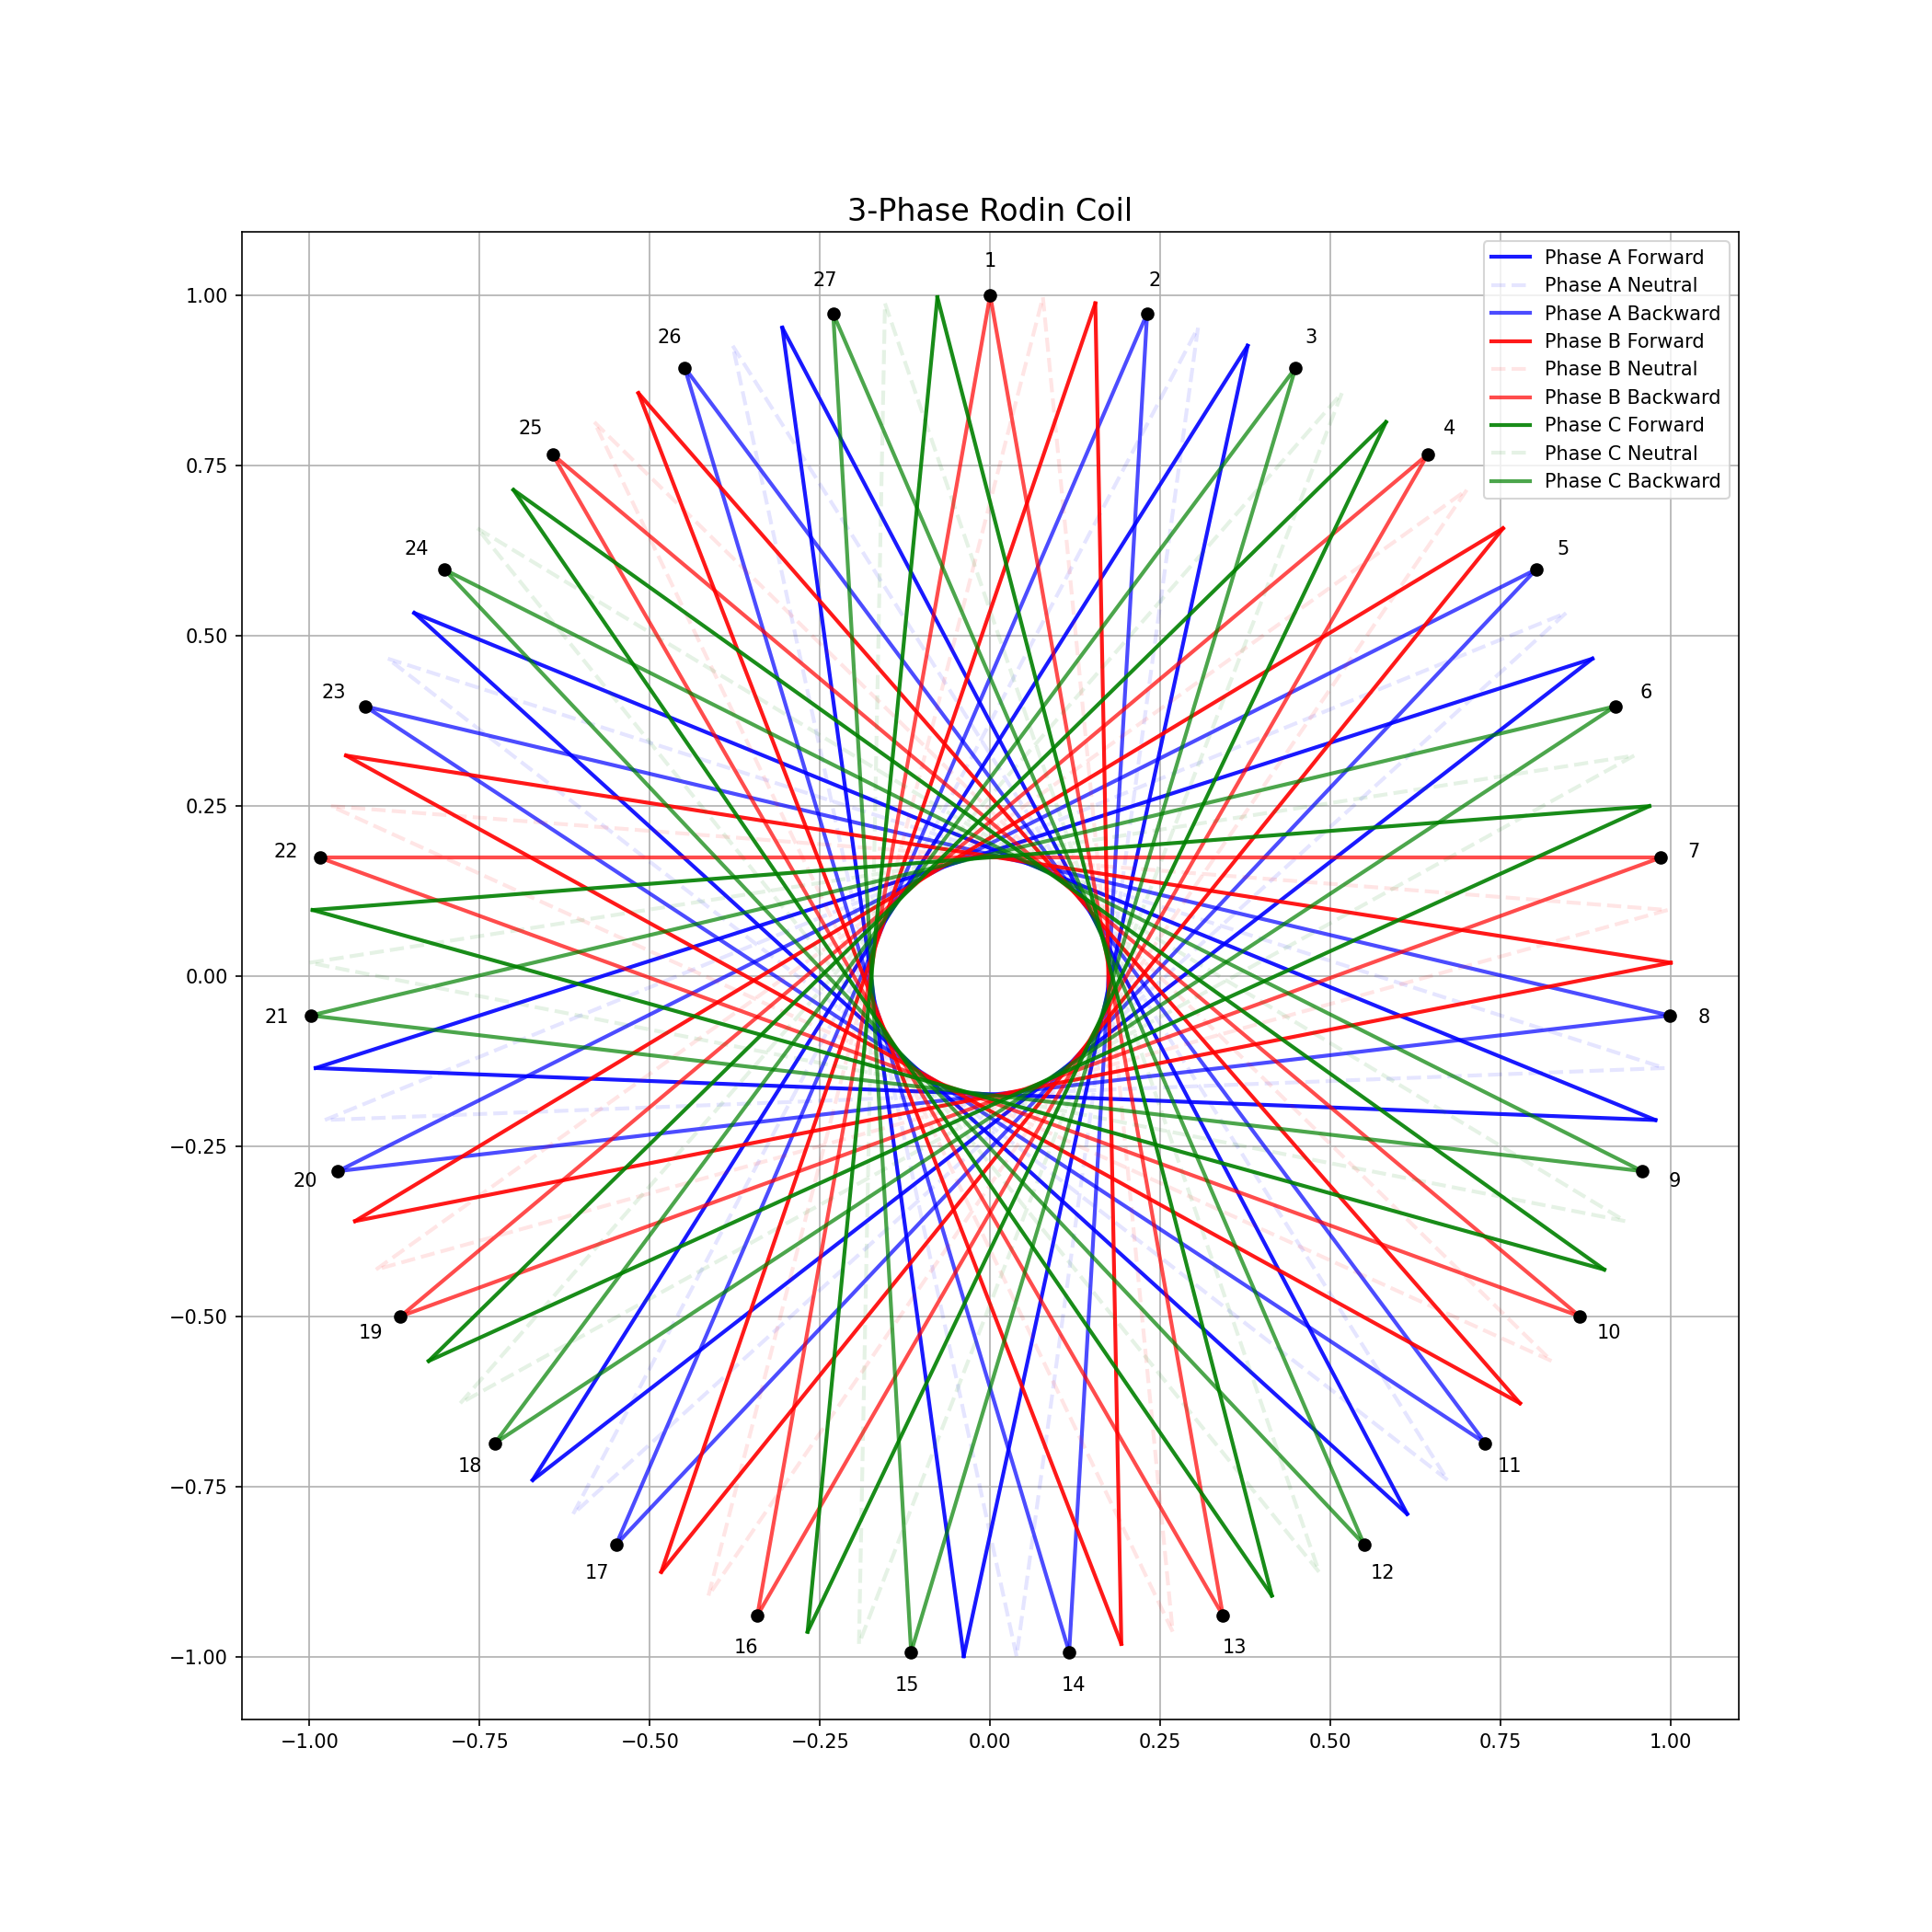
\includegraphics[width=0.5\textwidth]{exports/02_Starship-3phase-27x3points_030557}
\caption{Proposed coil resonance experiment: A multi-turn Rodin “starship” coil (black curve) is positioned between two coaxial magnet rings (blue = bottom ring, red = top ring) forming a vortex–antivortex pair. The magnets provide a static swirl field, while 3-phase currents in the coil drive a rotating aetheric vortex.}
\end{figure}


The first configuration employs a dual Rodin-style 3-phase coil arrangement inspired by the uploaded \textit{MagneticCircleRodin.py} design. As illustrated above, it consists of a specially wound toroidal coil (a “Rodin starship” coil) sandwiched between two parallel rings of permanent magnets oriented as a vortex–antivortex dipole. The magnet rings establish a steady baseline swirl field: e.g. the bottom ring (blue arrows) might produce a clockwise circulation in the local æther, while the top ring (red arrows, inverted orientation) induces a counter-clockwise swirl above – together mimicking a contained vortex/anti-vortex field loop. This static field provides a non-zero $\mathcal{S}_{\mu\nu}^{(0)}$ curvature background (analogous to a constant gravitational field) within the coil’s volume.


Through the Rodin coil, we then drive a 3-phase alternating current at frequency $f$, injecting a rotating magnetic field that couples to the aether fluid. The three evenly phase-shifted currents produce a continuously rotating B-field in the toroidal core region (much like a motor stator), thereby stirring the aether in a cyclical manner. At the design frequency $f \approx f_\textrm{res}$ (tuned so that the azimuthal propagation of the induced swirl matches $\lambda_\textrm{res}$ above), the coil’s field constructively pumps the aether’s swirl mode. In essence, the coil generates a dynamic vortex whose phase velocity matches the static field’s swirl phase – this resonance should greatly amplify the aether’s response.


Predicted Effects: When the coil’s swirl is \textit{anti-phase} to the static swirl (half a period out of phase), it will partially cancel the net curvature in the mid-plane. In VAM terms, the oscillating part $\delta \mathcal{S}_{\text{\mu\nu}}(\omega)$ subtracts from the static $\mathcal{S}_{\mu\nu}^{(0)}$ in that region, yielding a local shallowing of the æther pressure well that objects experience. A test mass suspended at the apparatus center or on a sensitive scale directly above the coil should lose weight (gravitation effectively shielded) during resonance peaks. Conversely, if the coil’s current phasing is adjusted $180^\circ$ (so that its swirl adds in-phase), the local curvature deepens and the test mass would gain slight weight. Detection of both regimes by adjusting phase/frequency would be a striking confirmation of controllable gravitational coupling. We anticipate only very small fractional weight changes ($\Delta g/g \ll 10^{-6}$), but modern gravimeters and force balances might detect them given sufficient signal integration. Notably, any nonlinear threshold behavior should be recorded: VAM predicts that beyond a certain swirl intensity (when aether drag forces approach the maximum $F_{\æ}^{\max}\approx29~\text{N}$ per vortex core), the æther may enter a new regime of reduced coupling – akin to a critical field in superconductors where magnetic flux is expelled. If such a threshold exists, one would see an abrupt change in weight at a certain coil current amplitude or power input, signaling the onset of the Meissner-like gravity expulsion (as suggested in VAM’s superconductivity analogy\VAMref{VAM-5}).


Another signature is clock rate modulation. Inside the coil’s active region, proper time $\tau$ should be altered by the oscillatory swirl. VAM’s time dilation law ($d\tau/dt = \sqrt{ 1-|\mathbf{v}\textit{\text{swirl}|^2/c^2}}$)\VAMref{VAM-1} indicates that when swirl velocity $|\mathbf{v}{\text{swirl}}|$ is reduced, clocks run faster, and when it is enhanced, clocks slow down. Thus during anti-phase resonance (weaker swirl), any clock or atomic frequency reference placed in the field should tick slightly faster relative to a reference clock outside the apparatus, and vice versa for in-phase driving (slower ticking due to extra swirl energy). We can interpret this as the swirl-clock phase $S(t)$ being modulated by the coil’s fields – effectively the device would create a small oscillating \textit{time dilation well}. The expected magnitude (perhaps $\Delta \nu/\nu \sim10^{-15}$ or less for microwave frequencies) is extremely tiny, but not inconceivable to measure with today’s ultra-stable atomic clocks or laser interferometric time comparison, especially by integrating over many cycles. Detection of a periodic modulation in clock rate synchronized to the coil current (and disappearing when $f$ is off-resonance) would strongly support the VAM model of gravity as an emergent swirl effect.


In summary, the dual-ring Rodin coil experiment serves as a direct test of aetheric frame-dragging and gravity control. It exploits a magnetic-induced vortex to interfere with Earth’s own swirl field. Observable outcomes would include: (i) \textit{Weight anomalies} (periodic or DC offset in apparent weight) of a test mass in the field, on the order of micro-g or less; (ii) \textit{Temporal frequency shifts} between clocks inside and outside the vortex region, in phase with the coil drive; and (iii) a possible \textit{nonlinear jump} in these effects once the input power crosses a threshold (indicating the aether vortex has reached a critical intensity for decoupling). Any positive findings – even a ppm-level weight change or $10^{-18}$-fraction clock shift – under controlled conditions (reversible by detuning $f$ or coil phase) would provide empirical evidence of the VAM’s core prediction that gravity can be modulated via engineered swirl fields\VAMref{VAM-2},\VAMref{VAM-10}.


\section*{Swirl-Mode Capacitor (Oscillating Dipole Plates)}

Our second proposed configuration uses oscillating electric fields to excite aether swirl modes, providing a conceptually distinct route to gravitational modulation. Consider a high-voltage parallel-plate capacitor oriented vertically, creating a strong electric dipole field in the space between the plates. If we apply an AC voltage that oscillates at frequency $f$, the electric field $\mathbf{E}(t)$ between the plates will reverse direction periodically. This time-varying dipole can be likened to a driven antenna for the aether: a changing $\mathbf{E}$ induces a circulating magnetic field ($\nabla\times \mathbf{E}\rightarrow -\partial \mathbf{B}/\partial t$), and in VAM the electromagnetic fields correspond to underlying aether vorticity and helicity patterns. Thus, an oscillating capacitor effectively pumps the aether fluid back-and-forth, and at the right frequency it can inject \textit{swirl waves} into the surrounding medium.


To maximize the swirl induction, the capacitor plates can be driven in synchrony with specific swirl eigenmodes of the system. For example, beyond the simple up-down field oscillation, one could use multiple segmentations of the plates or an array of phased electrodes to produce a rotating dipole moment (mimicking a higher-order swirl mode). By selecting the harmonic mode that matches $\lambda_\textrm{res}$, the rotating or oscillating electric field will resonate with an aether vortex pattern between the plates. In practice, one might use four quadrant electrodes driven $90^\circ$ out of phase (to rotate the field vector in the plane), or even a ring of capacitors triggered sequentially, to excite a circulating polarization in the aether. The notion of \textit{swirl-mode harmonics} here refers to these structured field oscillations (dipole, quadrupole, etc.) that couple to quantized circulation modes of the aether fluid. At resonance, the aether’s response – a whirl of polarization current and accompanying pressure field – is greatly amplified.


Predicted Effects: The oscillating dipole field will modulate the local aether density and pressure between the plates. According to VAM, regions of oscillatory pressure (due to the electric field’s energy density oscillations) can lead to modulations in $\mathcal{S}_{\text{00}}$ similar to a gravitational potential wave. If tuned to resonance, the aether inside the capacitor experiences a standing wave of swirl: when the field is in one direction, a slight under-density of aether (lower pressure) might form along the axis, and half a cycle later an over-density (higher pressure) forms, etc. This effectively creates an \textit{oscillating gravity well} along the dipole axis. A small test mass suspended between the plates would feel an alternating force – \textit{a transient weight change at frequency $f$}. While the rapid oscillation might average out to zero net weight change over a full cycle, any non-linearities or rectification in the aether response could produce a steady bias in weight. In particular, VAM suggests the possibility of time-averaged gravity shielding if the aether’s response to upward vs. downward field is asymmetric. For instance, if the fluid “slips” more easily in one half-cycle (reducing effective density more) than the other, the object would experience a net buoyancy over time. Detecting a tiny reduction in weight (e.g. via a torsion balance or superconducting gravimeter) when the capacitor is driven at $f\textrm{res}$, and not at off-resonant frequencies, would signal a real aether-mediated gravity modulation.


Additionally, time dilation effects are expected analogous to the coil case. The strong oscillating $\mathbf{E}$ field stores and releases energy each half-cycle, which in VAM corresponds to fluctuations in local aether energy density $\rho_{\æ}(t)$. Higher energy density (when field is maximum) means a locally lower proper time rate (slower clock), whereas lower energy (field passes through zero) means faster clock. An atomic clock placed between the plates and synchronized to the drive could look for a small periodic phase modulation of its ticking. The swirl-clock phase $S(t)$ in the aether between the plates will oscillate, producing a measurable beat note or sidebands in the clock signal if the effect is within sensitivity. Techniques like Ramsey interferometry or comparing two identical atomic clocks (one inside the field, one outside) over many oscillation cycles might reveal this differential ticking. Though the magnitude is likely extremely small (perhaps a fractional frequency shift of order $10^{-16}$ on a fast $f\sim$ MHz–GHz drive), it is in principle detectable given current clock precision (which has reached $10^{-18}$ stability).


Resonant Power Thresholds: Just as with the coil setup, the capacitor experiment may exhibit threshold behavior. At low drive voltages, the aether essentially oscillates linearly (small perturbation), and any gravity modulation will be proportional to input power. However, if the drive voltage is increased, the aether swirl amplitude grows; once the swirl’s inertial forces approach the internal æther stress limit (set by $C_e$, $\rho_{\æ}^\textrm{(fluid)}$, etc.), the system could enter a non-linear regime. VAM posits a maximum sustainable vorticity and force density in the æther (e.g. a maximum circulation or a breaking of laminar flow beyond some point). When this happens, additional input energy goes into reorganizing the flow (perhaps forming quantized vortex filaments or expelling swirl out of the region) rather than increasing local curvature. The experimental tell-tale would be a saturation or sudden drop in the gravity-coupling effect despite rising input power. In practical terms: as the AC voltage is ramped up, one might see the test mass weight reduction deepen and then plateau (or even reverse if swirl is expelled) above a certain field strength. Documenting such a threshold would reinforce the analogy to superconductors (with the voltage threshold akin to critical field for Meissner effect) and highlight the inherently non-linear nature of the aether fluid.


Summary of Signatures: The oscillating-capacitor approach offers a more purely electrostatic route to test VAM. Key expected signals include:


\begin{itemize}

\item
Periodic weight fluctuations of a test mass in the field at the drive frequency (e.g. observable via a spectrum analyzer on a weight sensor), and possibly a small DC offset in apparent weight when on resonance.




\item
Clock phase drifts or modulation synchronized to the field oscillation, detectable by high-precision timing.




\item
Resonance sharpness and threshold: a pronounced increase in effect magnitude when $f$ hits the calculated $\lambda_\textrm{res}$ (scan the frequency and look for a peak response), and a non-linear response as drive amplitude passes a critical level (indicating aether flow restructuring).




\end{itemize}

Both experimental configurations target a core falsifiable outcome: the existence of an adjustable, harmonic coupling to gravity. According to VAM, gravity is not a static geometry but an emergent, frequency-dependent phenomenon – by tuning into the aether’s swirl modes, we can, in principle, \textit{open or close} the coupling to gravity in a local region. A positive detection (even if small) of gravity modulation at a specific resonant frequency, along with the predicted phase-dependent reversibility (enhancement vs. suppression), would confirm VAM’s most provocative predictions~\VAMref{VAM-2},\VAMref{VAM-15}. It would mark the first empirical evidence that the “stiffness” of spacetime (in Newton’s terms) can be modulated like a medium – validating the fluidic paradigm of VAM and opening a new frontier in gravitational control technology.








\begin{thebibliography}{99}

    \bibitem{Podkletnov1992}
    E. Podkletnov and R. Nieminen, “A possibility of gravitational force shielding by bulk YBa$_2$Cu\textit{3$O$}{7-x} superconductor,” \emph{Physica C}, vol. 203, no. 3-4, pp. 441–444, 1992.

    \bibitem{Barcelo2011}
    C. Barceló, S. Liberati, and M. Visser, “Analogue Gravity,” \emph{Living Reviews in Relativity}, vol. 14, no. 3, 2011.

    \bibitem{Everitt2011}
    C. W. F. Everitt \emph{et al.}, “Gravity Probe B: Final Results of a Space Experiment to Test General Relativity,” \emph{Phys. Rev. Lett.}, vol. 106, p. 221101, 2011.


    \bibitem{VAM-0}\label{VAM-0}
    O. Iskandarani,
    \emph{“Revisiting the Æther:  From Einstein to the Vortex Fluid Paradigm”}\\
    {\scriptsize VAM-0 preprint (2025).
    \href{https://doi.org/10.5281/zenodo.15669901}{\texttt{DOI:10.5281/zenodo.15669901}}}


    \bibitem{VAM-1}\label{VAM-1}
    O. Iskandarani,
    \emph{“Time Dilation in a 3D Superfluid Æther Model”}\\
    {\scriptsize VAM-1 preprint (2025).
    \href{https://doi.org/10.5281/zenodo.15669794}{\texttt{DOI:10.5281/zenodo.15669794}}}

    \bibitem{VAM-2}\label{VAM-2}
    O. Iskandarani,
    \emph{“Swirl Clocks and Vorticity-Induced Gravity: Reformulating Relativity in a Structured Vortex Æther”}\\
    {\scriptsize VAM-2 preprint (2025).
    \href{https://doi.org/10.5281/zenodo.15566335}{\texttt{DOI:10.5281/zenodo.15566335}}}

    \bibitem{VAM-3}\label{VAM-3}
    O. Iskandarani,
    \emph{“Benchmarking the Vortex Æther Model Against General Relativity”}\\
    {\scriptsize VAM-3 preprint (2025).
    \href{https://doi.org/10.5281/zenodo.15665432}{\texttt{DOI:10.5281/zenodo.15665432}}}

    \bibitem{VAM-4}\label{VAM-4}
    O. Iskandarani,
    \emph{“Emergent General Relativity from Structured Swirl Dynamics in the Vortex Æther Model”}\\
    {\scriptsize VAM-4 preprint (2025).
    \href{https://doi.org/10.5281/zenodo.15712577}{\texttt{DOI:10.5281/zenodo.15712577}}}

    \bibitem{VAM-5}\label{VAM-5}
    O. Iskandarani,
    \emph{“On a Vortex-Based Lagrangian Unification of Gravity and Electromagnetism”}\\
    {\scriptsize VAM-5 preprint (2025).
    \href{https://doi.org/10.5281/zenodo.15772857}{\texttt{DOI:10.5281/zenodo.15772857}}}

    \bibitem{VAM-6}\label{VAM-6}
    O. Iskandarani,
    \emph{“Knotted Gauge Fields: Rebuilding the Standard Model from Vortex Æther Dynamics”}\\
    {\scriptsize VAM-6 preprint (2025).
    \href{https://doi.org/10.5281/zenodo.15772832}{\texttt{DOI:10.5281/zenodo.15772832}}}

    \bibitem{VAM-7}\label{VAM-7}
    O. Iskandarani,
    \emph{“From Quantum Constants to Galactic Swirl: Deriving Æther Density in the VAM Framework”}\\
    {\scriptsize VAM-7 preprint (2025).
    \href{https://doi.org/10.5281/zenodo.15701958}{\texttt{DOI:10.5281/zenodo.15701958}}}

    \bibitem{VAM-8}\label{VAM-8}
    O. Iskandarani,
    \emph{“The Vortex Æther Model: A Unified Topological Field Theory of Mass, Gravity, and Time”}\\
    {\scriptsize VAM-8 preprint (2025).
    \href{https://doi.org/10.5281/zenodo.15848010}{\texttt{DOI:10.5281/zenodo.15848010}}}

    \bibitem{VAM-9}\label{VAM-9}
    O. Iskandarani,
    \emph{“Milky Way as a Chiral Swirl-Knot Network – Exclusion of Achiral Knots”}\\
    {\scriptsize VAM-9 preprint (2025).
    \href{https://doi.org/10.5281/zenodo.15870399}{\texttt{DOI:10.5281/zenodo.15870399}}}

    \bibitem{VAM-10}\label{VAM-10}
    O. Iskandarani,
    \emph{“Swirl-Induced Curvature as the Mechanism of Gravitation in the Vortex Æther Model”}\\
    {\scriptsize VAM-10 preprint (2025).
    \href{https://doi.org/10.5281/zenodo.15870448}{\texttt{DOI:10.5281/zenodo.15870448}}}

    \bibitem{VAM-11}\label{VAM-11}
    O. Iskandarani,
    \emph{“Master Equation for Particle Masses”}\\
    {\scriptsize VAM-11 preprint (2025).
    \href{https://doi.org/10.5281/zenodo.16324153}{\texttt{DOI:10.5281/zenodo.16324153}}}

    \bibitem{VAM-12}\label{VAM-12}
    O. Iskandarani,
    \emph{“Fractal Swirl Extension of the Vortex Æther Model”}\\
    {\scriptsize VAM-12 preprint (2025).
    \href{https://doi.org/10.5281/zenodo.16324782}{\texttt{DOI:10.5281/zenodo.16324782}}}

    \bibitem{VAM-13}\label{VAM-13}
    O. Iskandarani,
    \emph{“Beyond Spacetime: A Fluid-Dynamic Theory of Gravity and Time from Vorticity”}\\
    {\scriptsize VAM-13 preprint (2025).
    \href{https://doi.org/10.5281/zenodo.15706546}{\texttt{DOI:10.5281/zenodo.15706546}}}

    \bibitem{VAM-14}\label{VAM-14}
    O. Iskandarani,
    \emph{“Topological \& Fluid-Dynamic Lagrangian in the Vortex Æther Model”}\\
    {\scriptsize VAM-14 preprint (2025).
    \href{https://doi.org/10.5281/zenodo.16325219}{\texttt{DOI:10.5281/zenodo.16325219}}}

    \bibitem{VAM-15}\label{VAM-15}
    O. Iskandarani,
    \emph{“Quantum Mechanics and Quantum Gravity in the Vortex Æther Model: A Reformulation Using Superfluid Vorticity and Topology”}\\
    {\scriptsize VAM-15 preprint (2025).
    \href{https://doi.org/10.5281/zenodo.15870859}{\texttt{DOI:10.5281/zenodo.15870859}}}







\end{thebibliography}





\end{document}



